\subsubsection{Exponentially Weighted Moving Average} \label{link::ewma}
Предполагаем, что в наличии есть данные о некотором показателе $\theta_t: t = \overline{1,n}$. В данный момент перед нами не стоит задача предсказания следующего показателя, нужно только визуально выявить тренд, чтобы приблизительно понять направление движение показателя в осях (время, значение). Конечно, в этой формулировке отсутствует строгость, пока что останавливаемся на том, что есть. Экспоненциальная скользящая средняя занимается тем, что уже заложено в ее названии: сглаживает показатели посредством усреднения. То есть в текущем значении ($t$) используется как значение в предыдущий момент времени ($t - 1$), так и значение наблюдения в момент времени ($t$). Иными словами, получается выпуклая линейная комбинация текущего и предыдущего значений:
\begin{equation}
	v_t = \beta \cdot v_{t - 1} + (1 - \beta) \cdot \theta_t: \; \beta \in (0,1)
\end{equation}
Где $\beta$ - показатель, пропорциональный примерному количеству дней, по которым происходит усреднение, а $v_0 = 0$ - первое значение экспоненциальной скользящей средней. Для изучения данного рекуррентного соотношения "раскручиваем"\ его в обратном направлении:
\begin{equation}
	\begin{split}
		v_t & =  (1 - \beta) \cdot \theta_t + \beta \cdot \overbrace{\left\{(1 - \beta) \theta_{t - 1} + \beta v_{t - 2}\right\}}^{v_{t - 1}}\\
		& =  (1 - \beta) \cdot \theta_t + \beta \cdot \{(1 - \beta) \cdot \theta_{t - 1} + \beta \cdot \overbrace{\left\{(1 - \beta) \cdot \theta_{t - 2} + \beta \cdot v_{t - 3}\right\}}^{v_{t - 2}}\}\\
	\end{split}
\end{equation}
Для лучшего понимания, рассматриваем частный случае:
\begin{equation}
	\begin{split}
		v_4 & = \beta \cdot v_3 + (1 - \beta) \cdot \theta_4\\
		v_3 & = \beta \cdot v_2 + (1 - \beta) \cdot \theta_3\\
		v_2 & = \beta \cdot v_1 + (1 - \beta) \cdot \theta_2\\
		v_1 & = \beta \cdot v_0 + (1 - \beta) \cdot \theta_1\\
		v_0 & = 0
	\end{split}
\end{equation}
Тогда:
\begin{equation}
	\begin{split}
		v_4 & =  (1 - \beta) \theta_4 + \beta ((1 - \beta) \theta_3 + \beta ((1 - \beta) \theta_2 + \beta((1 - \beta) \theta_1 + \overbrace{\beta \cdot 0}^{v_0 = 0})))\\
		& = (1 - \beta) \theta_4 + (1 - \beta) \beta \cdot \theta_3 + (1 - \beta) \beta^2 \cdot \theta_2 + (1 - \beta) \beta^3 \cdot \theta_1\\
		& = (1 - \beta) \sum_{t = 1}^4 \beta^{4 - t} \cdot \theta_t
	\end{split}
\end{equation}
Аналогично происходит раскрытие и для больших показателей $v_n$. А значит, получается формула вида:
\begin{equation}
	v_n = (1 - \beta) \sum_{t = 0}^n \beta^t \cdot \theta_{n - t}
\end{equation}
Отсюда качественно делаем вывод, что последним значениям наблюдаемого показателя ($\theta$) соответствует большее значение коэффициента, то есть чем ближе $\theta_{t}$ к $v_n$ с точки зрения индекса, тем больше при нем коэффициент. Теперь, возвращаясь к названию модели, отмечаем, что она должна усреднять по конкретному количеству временных единиц, следовательно, $\beta$ (единственный гиперпараметр) должен регулировать указанный показатель (то есть количество дней, по которым происходит усреднение). Обычно, рассматривается следующее соотношение: $\beta = 1 - \alpha / (N + 1)$, где $N$ - количество дней, а $\alpha$ - фактор сглаживания. Опираясь на \cite{ewma}, полагаем $\alpha = 2$ как наиболее распространенное значение.

Далее рассматриваем подробнее первые значения EWMA, а конкретнее - для лучшего осознания - самое первое: $v_0 \Rightarrow v_1 = (1 - \beta) \cdot \theta_1 \Rightarrow$ при $\beta \to 1 - 0$ получаем, что $(1 - \beta) \cdot \theta_1 \ll \theta_1$, что крайне плохо отражается на самих значениях. Таким образом, вычленение тренда становится более трудным на начальных этапах из-за плохого "разогрева"\ модели. Данная проблема называет bias (смещение), а ее решение bias correction (коррекция смещения) соответственно. Основой подобной корректировки является множитель вида $(1 - \beta^t)$. Очевидно, что при $\beta \in (0,1)$, а именно так и есть по построению, $\lim\limits_{t \to +0}(1 - \beta^t) = 0$, а $\lim\limits_{t \to +\infty}(1 - \beta^t) = 1$.
\begin{equation}
	\begin{split}
		v_n & = (1 - \beta^n)^{-1} \cdot (\beta \cdot v_{n - 1} + (1 - \beta) \cdot \theta_n)\\
		v_n & = (1 - \beta^n)^{-1} \cdot (1 - \beta) \left(\sum_{t = 0}^n \beta^t \cdot \theta_{n - t}\right)
	\end{split}
\end{equation}
Тогда на начальных этапах коррекция выравнивает ранее сильно уменьшенные значения EWMA, а на последующих (при $n \to \infty$) ее влияние ослабеваем, постепенно сводясь к 0 (то есть - делению на 1). Данный способ занимает очень мало памяти компьютера, так как для вычисления ему всегда необходимо хранить только 2 переменные: $v_t$ и $\beta$.

Иллюстрируем вышеизложенную теорию на примере реальных данных. Рассматривается цена открытия акций компании Apple за 2021 год. Первоначально сами значения, представленные в координатах ($t$ - месяц года, $y_t$ - цена в рублях), имеют вид:
\begin{figure}[H]
	\centering
	\begin{tikzpicture}
		\begin{axis}[
			grid = both,
			legend pos = north west,
			minor tick num = 1,
			major grid style = {lightgray},
			minor grid style = {lightgray!25},
			xlabel = {2021 год},
			width = \textwidth,
			height = 0.5 \textwidth,
			xmin=-5, xmax=260,
			ymin=115, ymax=185,
			xtick={0, 40, 80, 120, 160, 200, 240},
			xticklabels={03/01, 02/03, 28/04, 24/06, 20/08, 18/10, 14/12},
			line width=0.3mm
			]
			\addplot table [
			x=x, 
			y=Open, 
			col sep=comma,
			mark={},
			] {./source/source_csv/Illustration data/apple_data_test.csv};
			\legend{AAPL 2021}
		\end{axis}
	\end{tikzpicture}
	\caption{Цены открытия акций Apple (AAPL) 2021 (руб.)}
\end{figure}
Исходя из графика, получаем, что данные очень нестабильны, то есть с первого взгляда невозможно точно сказать, каков тренд. Однако в общих чертах графика однозначно видно, что от малых значений цен показатели переходят к б\'{о}льшим. Применяем к данным модель EWMA.
\begin{figure}[H]
	\centering
	\begin{tikzpicture}
		\begin{axis}[
			grid = both,
			legend pos = north west,
			minor tick num = 1,
			major grid style = {lightgray},
			minor grid style = {lightgray!25},
			xlabel = {2021 год},
			width = \textwidth,
			height = 0.5 \textwidth,
			xmin=-5, xmax=260,
			ymin=115, ymax=185,
			xtick={0, 40, 80, 120, 160, 200, 240},
			xticklabels={03/01, 02/03, 28/04, 24/06, 20/08, 18/10, 14/12},
			line width=0.3mm
			]
			\addplot table [
			x=x, 
			y=Open, 
			col sep=comma,
			mark={},
			] {./source/source_csv/Illustration data/apple_data_test_ewma.csv};
			%\legend{AAPL 2021};
			
			\addplot table [
			x=x, 
			y=V_2, 
			col sep=comma,
			mark={},
			] {./source/source_csv/Illustration data/apple_data_test_ewma.csv};
			%\legend{EWMA $\beta = 0.1$};
			
			
			\addplot table [
			x=x, 
			y=V_10, 
			col sep=comma,
			mark={},
			] {./source/source_csv/Illustration data/apple_data_test_ewma.csv};
			%\legend{EWMA $\beta = 0.1$};
			
			\addplot table [
			x=x, 
			y=V_30, 
			col sep=comma,
			mark={},
			] {./source/source_csv/Illustration data/apple_data_test_ewma.csv};
			%\legend{EWMA $\beta = 0.3$};
			
			\addplot table [
			x=x, 
			y=V_50, 
			col sep=comma,
			mark={},
			] {./source/source_csv/Illustration data/apple_data_test_ewma.csv};
			%\legend{EWMA $\beta = 0.5$};
			
			
			\addplot table [
			x=x, 
			y=V_90, 
			col sep=comma,
			mark={},
			] {./source/source_csv/Illustration data/apple_data_test_ewma.csv};
			%\legend{EWMA $\beta = 0.9$};
			
			\addplot table [
			x=x, 
			y=V_200, 
			col sep=comma,
			mark={},
			] {./source/source_csv/Illustration data/apple_data_test_ewma.csv};
			%\legend{EWMA $\beta = 0.9$};
			
			\legend{AAPL 2021, $n = 2$, $n = 10$, $n = 30$, $n = 50$, $n = 90$, $n = 200$};
		\end{axis}
	\end{tikzpicture}
	\caption{EWMA, цены открытия AAPL 2021 (руб.)}
\end{figure}
Глядя на полученный результат сразу ясно, что тренд восходящий, однако это предположение делается только на основе визуального анализа. Пока что никаких алгоритмов нет. Однако нельзя недооценивать полученную информацию, так как более явный тренд позволяет моделям (нейронных сетей) более точно настраиваться на обучающую выборку, что часто приводит к улучшению результату предсказаний (если, конечно не довести до переобучения: данные термины и теория объясняется в блоке \myref{link::neural_networks}). Также стоит отметить всплеск, случившийся при $n = 2$. Это произошло именно именно из-за технических особенностей добавленного множителя, корректирующего смещение. 

Последним пунктом необходимо рассказать более подробно о самом корректирующем множителе. \textbf{Q}: Почему у него именно такой вид, ведь можно просто сделать первое значение таким же, как в исходном ряде? \textbf{A}: 1) необходимо корректировать вычисления, исходя из одной формулы, так как цель - прийти именно к общности 2) при последующих наблюдения данный коэффициент становится чрезвычайно малым $\lim\limits_{t \to +\infty}(1 - \beta^t) = 1$, а при первоначальных значениях не оказывает влияния $\lim\limits_{t \to +0}(1 - \beta^t) = 0$. Однако при индексах (речь о непрерывных), стремящихся к $0$, обратная величина стремится к $\infty$, что очень плохо с вычислительной точки зрения, так как у компьютера может произойти переполнение памяти и вместо числа получится NaN или Null, что не позволит далее осуществлять расчеты. Поэтому в начале графике наблюдается резкий всплеск, сходящийся впоследствии к исходному ряду. Далее приводится график значений корректирующих коэффициентов в зависимости от $\beta$ и от $t$.
\begin{figure}[H]
	\centering
	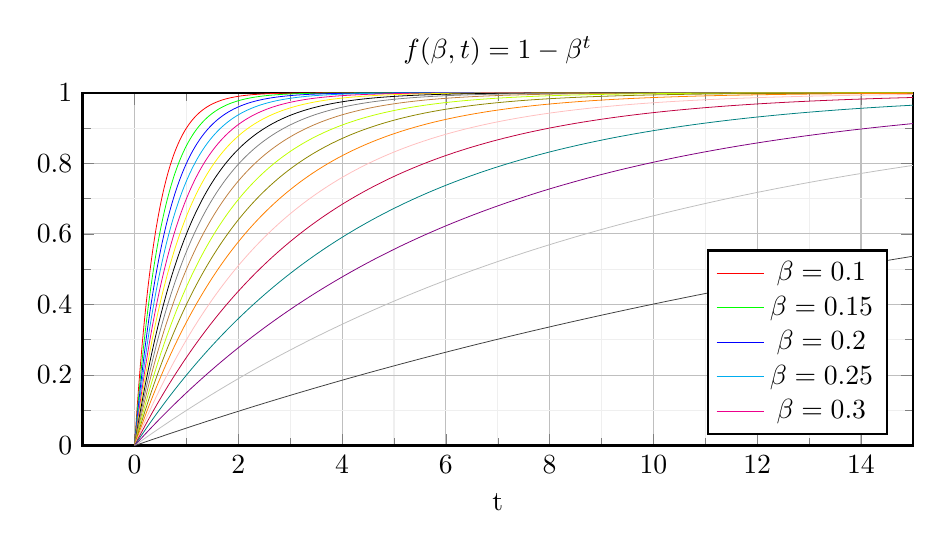
\begin{tikzpicture}
		\begin{axis}[
			grid = both,
			legend pos = south east,
			minor tick num = 1,
			major grid style = {lightgray},
			minor grid style = {lightgray!25},
			title={$f(\beta, t) = 1 - \beta^t$},
			xlabel = {t},
			width = \textwidth,
			height = 0.5 \textwidth,
			xmin=-1, xmax=15,
			ymin=0, ymax=1,
			%xtick={0, 40, 80, 120, 160, 200, 240},
			%xticklabels={03/01, 02/03, 28/04, 24/06, 20/08, 18/10, 14/12},
			line width=0.3mm
			]
			\addplot[domain = 0:15,
			samples = 300,
			color = red,
			smooth,
			line width = 0.01cm,] {1 - 0.1^x};
			\addplot[domain = 0:15,
			samples = 300,
			color = green,
			smooth,
			line width = 0.01cm,] {1 - 0.15^x};
			\addplot[domain = 0:15,
			samples = 300,
			color = blue,
			smooth,
			line width = 0.01cm,] {1 - 0.2^x};
			\addplot[domain = 0:15,
			samples = 300,
			color = cyan,
			smooth,
			line width = 0.01cm,] {1 - 0.25^x};
			\addplot[domain = 0:15,
			samples = 300,
			color = magenta,
			smooth,
			line width = 0.01cm,] {1 - 0.3^x};
			\addplot[domain = 0:15,
			samples = 300,
			color = yellow,
			smooth,
			line width = 0.01cm,] {1 - 0.35^x};
			\addplot[domain = 0:15,
			samples = 300,
			color = black,
			smooth,
			line width = 0.01cm,] {1 - 0.4^x};
			\addplot[domain = 0:15,
			samples = 300,
			color = gray,
			smooth,
			line width = 0.01cm,] {1 - 0.45^x};
			\addplot[domain = 0:15,
			samples = 300,
			color = brown,
			smooth,
			line width = 0.01cm,] {1 - 0.5^x};
			\addplot[domain = 0:15,
			samples = 300,
			color = lime,
			smooth,
			line width = 0.01cm,] {1 - 0.55^x};
			\addplot[domain = 0:15,
			samples = 300,
			color = olive,
			smooth,
			line width = 0.01cm,] {1 - 0.6^x};
			\addplot[domain = 0:15,
			samples = 300,
			color = orange,
			smooth,
			line width = 0.01cm,] {1 - 0.65^x};
			\addplot[domain = 0:15,
			samples = 300,
			color = pink,
			smooth,
			line width = 0.01cm,] {1 - 0.7^x};
			\addplot[domain = 0:15,
			samples = 300,
			color = purple,
			smooth,
			line width = 0.01cm,] {1 - 0.75^x};
			\addplot[domain = 0:15,
			samples = 300,
			color = teal,
			smooth,
			line width = 0.01cm,] {1 - 0.8^x};
			\addplot[domain = 0:15,
			samples = 300,
			color = violet,
			smooth,
			line width = 0.01cm,] {1 - 0.85^x};
			\addplot[domain = 0:15,
			samples = 300,
			color = lightgray,
			smooth,
			line width = 0.01cm,] {1 - 0.9^x};
			\addplot[domain = 0:15,
			samples = 300,
			color = darkgray,
			smooth,
			line width = 0.01cm,] {1 - 0.95^x};
			\legend{$\beta = 0.1$, $\beta = 0.15$, $\beta = 0.2$, $\beta = 0.25$, $\beta = 0.3$};
		\end{axis}
	\end{tikzpicture}
	\caption{График корректирующих коэффициентов}
\end{figure}
В трехмерном пространстве это выглядит так:
\begin{figure}[H]
	\centering
	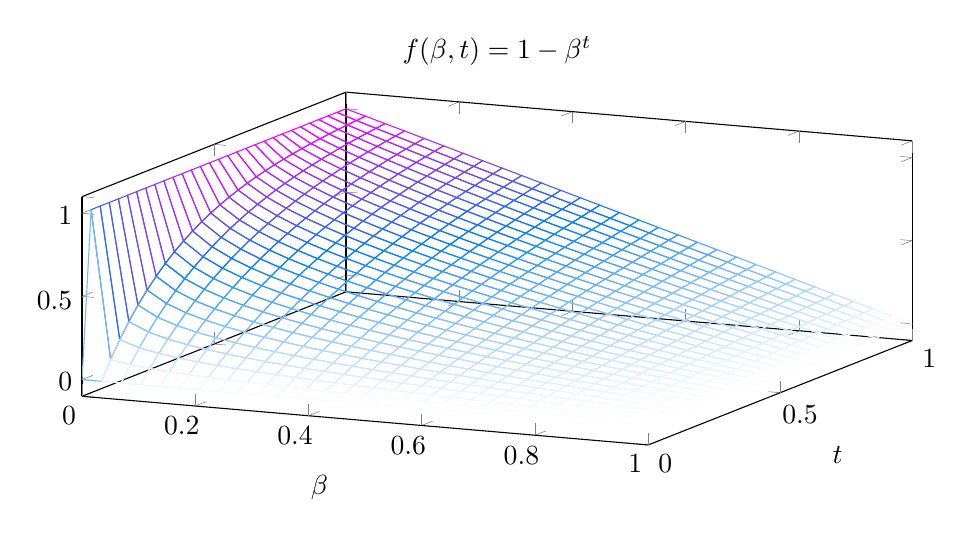
\begin{tikzpicture}
		\begin{axis}
			[
			title={$f(\beta, t) = 1 - \beta^t$},
			%hide axis,
			colormap/cool,
			width = \textwidth,
			height = 0.5 \textwidth,
			xlabel={$\beta$},
			ylabel={$t$}
			] 
			\addplot3[
			mesh,
			samples=30,
			domain=0:1,
			]{1 - x^y};
		\end{axis}
	\end{tikzpicture}
	\caption{Трехмерное изображение корректирующих коэффициентов}
\end{figure}
Данная модель является наиболее простой, однако она обладает возможностью предсказания.
\begin{equation}
	\begin{split}
		v_{t + 1} & = k \cdot y_t + (1 - k) \cdot v_t: \; k \in (0, 1)
	\end{split}
\end{equation}
В данном случае $v_t$ - это предсказанное значение на момент времени $t$. Модель не является устойчивой к наличию сезонности и тренду, однако факт того, что предсказания возможны есть. Значит, эта модель включается в список попадающих в сравнительную таблицу.
